\begin{figure}[htbp]
\centering
\caption{
  \textbf{An introduction to Modern Portfolio Theory mean-variance optimization.}
}
\label{fig:mpt}
\end{figure}

\clearpage

\begin{figure}[htbp]
\centering 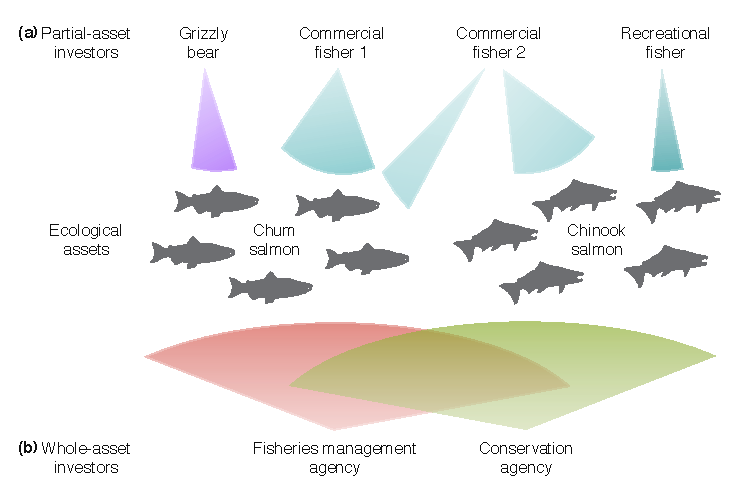
\includegraphics[width=5in]{salmon-portfolios.pdf} \caption{\textbf{There
  are multiple ways of investing in ecological portfolios.} In this example,
  investors are shown along the top and bottom and ecological assets are shown
  in the middle (populations of chum salmon, \textit{Oncorhynchus keta}, and
  Chinook salmon, \textit{Oncorhynchus tshawytscha}). The shaded arcs indicate
  investment. \textbf{(a)} Partial-asset investors invest by removing portions
  of the salmon populations --- the salmon that commercial fisher 1 removes are
  unavailable for the grizzly bear. These investors can often change their
  investment with ease. For example, commercial fisher 2 could decide to fish
  more Chinook and less chum salmon. Most financial portfolio theory is
  developed around this paradigm. \textbf{(b)} Whole-asset investors invest in
  entire populations. These investors can share assets but may have different
  goals for their portfolio. They can adjust their investment by managing
  properties of the population itself. For example, the fisheries management
  agency could reduce fishing of chum salmon to allow the population to grow.
  The conservation agency could fund habitat restoration for Chinook salmon to
  increase carrying capacity and expand their investment.}
\label{fig:salmonport}
\end{figure}

\begin{figure}[htbp]
\centering
%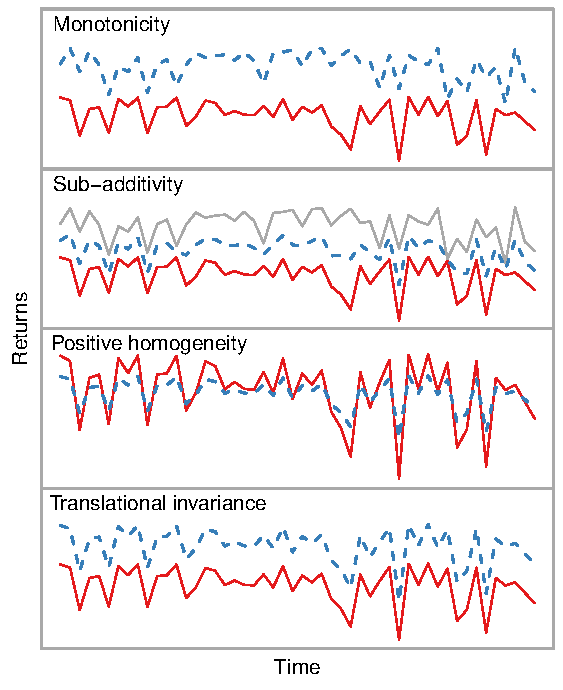
\includegraphics[width=2.6in]{coherence-axioms.pdf}
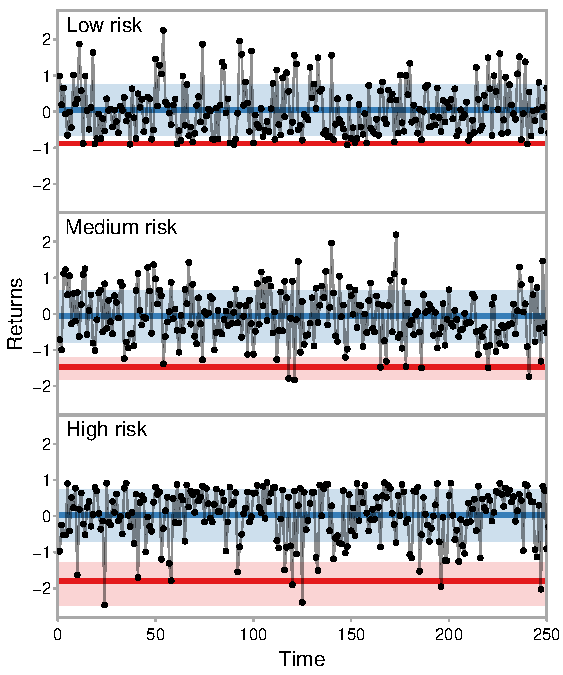
\includegraphics[height=3.0in]{skewness-abundance.pdf}
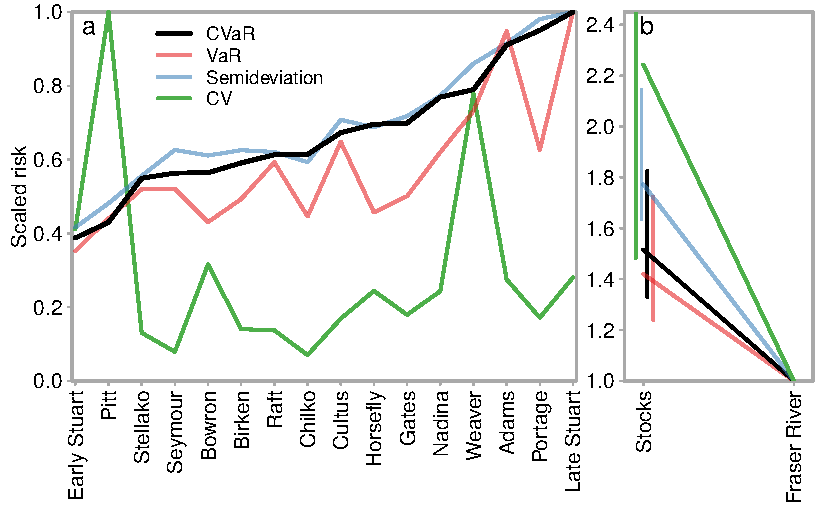
\includegraphics[height=2.0in]{compare-risk-and-portfolio-scale.pdf} \caption{
  \textbf{Symmetric vs.\ downside risk measures.} \textbf{(Left panel)} An
  illustration of three systems with similar properties of symmetric
  variability but different levels of risk. The y-axis denotes rate of change
  of abundance (``returns'' in financial terminology). The
  dark blue line represents the mean and the blue shaded region represents
  $\pm$ one standard deviation --- a measure that does not account for the
  assymetric property of risk. The red line represents the 95\% CVaR
  (conditional value at risk) and the red shaded region represents the region
  below the 95\% VaR (value at risk). CVaR and VaR are both downside risk
  measures that accurately identify higher risk systems. \textbf{(Right panel)}
  \textbf{(a)} Symmetric and downside risk metrics applied to annual returns of
  sockeye salmon stocks in the Fraser River. Stocks are ordered by increased
  CVaR. Symmetric (CV) and asymmetric (all other) risk metrics differ
  considerably in their rank order of risk for the different stocks.
  \textbf{(b)} The portfolio effect calculated for the same salmon stocks using
  the four risk metrics. Sloped lines at the stock level represent the mean
  portfolio effect and the vertical segments show the interquartile range.}
\label{fig:risk}
\end{figure}
